\documentclass{scrartcl}
\usepackage[utf8]{inputenc}
\usepackage{graphicx}
%opening
\title{Preinforme 2 - Laboratorio de Electrónica}

\author{
	\footnotesize Hernández A., Alejandro\\
	\footnotesize \texttt{a.hernandez105@uniandes.edu.co}
	\and
	\footnotesize Prada G., Jesús David\\
	\footnotesize \texttt{jd.prada1760@uniandes.edu.co}
       }
\date{\vspace{-5ex}}
%\date{}

\setlength{\parindent}{0pt}
\renewcommand{\indent}{\hspace*{\tindent}}

\begin{document}

\maketitle

\begin{abstract}
\small
En esta práctica de laboratorio se pretende aprender el funcionamiento experimental de elementos electrónicos tales como diodos, transistores y LEDs con el fin de reproducir mediante el uso de dichos elemementos el funcionamiento de compurtas lógicas y switches.
\end{abstract}

\section{Diodos}

Un diodo es un componente electrónico de dos terminales conconductancia asimétrica, esto es, permite el paso de corriente con resistencia nula en una dirección mientras que impide totalmente el paso de la misma en dirección opuesta.\\

Los diversos tipos de diodos que existen se muestran en la figura \ref{fig: diodos1}.

\begin{figure}[h!]
	\centering
	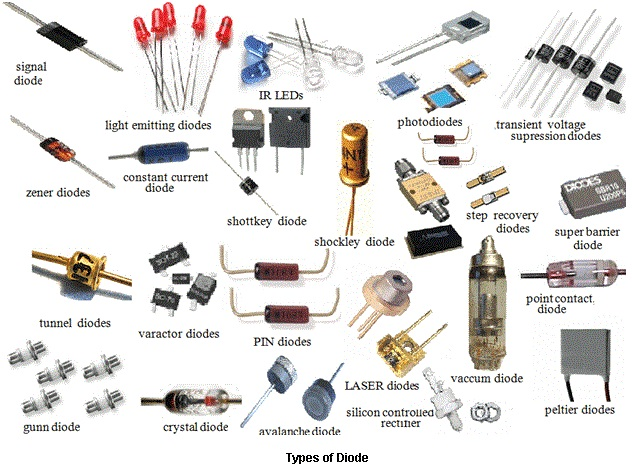
\includegraphics[width=0.85\textwidth]{diodos1}
	\caption{Tipos de diodos.}
	\label{fig: diodos1}
\end{figure}

\begin{figure}[h!]
	\centering
	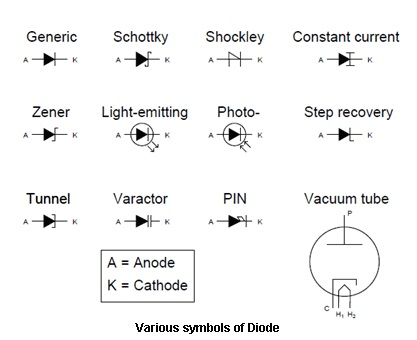
\includegraphics[width=0.6\textwidth]{diodos2}
	\caption{Tipos de diodos.}
	\label{fig: diodos2}
\end{figure}

Las características de los tipos de diodos más frecuentemente usados se describen a continuación:

\begin{itemize}
	\item \textbf{Diodos termoiónicos:} También llamados diodos de vacío, este tipo de diodos consisten básicamente de un arreglo de dos electrodos empacados al vacío dentro de una tubo de vidrio. Uno de los electrodos es un cátodo calentado por un filamento, el otro electrodo es una lámina (ánodo) y el voltaje alternante a ser rectificado es aplicado entre el cátodo y la lámina concéntrica. Cuando el cátodo es calentado, emite electrones al vacío por medio de un proceso llamado emisión termoiónica. Si la lámina tiene un voltaje positivo con respecto al cátodo, dicha lámina atrae electrostáticamente a los electrones, creando una corriente del cátodo a la lámina. En caso contrario, no se genera niguna corriente puesto que la lámina no atrae a los electrones.
	
	\item \textbf{Diodos semiconductores:} También denominados diodos de juntura, estos diodos se componen de un cristal semiconductor (como silicio o germanio) dopado con impurezas con el fin de generar dos regiones, a saber, una región que contenga portadores de carga negativa (electrones), llamada semiconductor de tipo n, y una región que contenga portadores de carga positiva (huecos), llamada seminconductor tipo p. Cuando las dos zonas se unen a través de las terminales del diodo (juntura p-n) un flujo momentáneo de electrones ocurre de la región n a la región p, dando como resultado una tercera zona, llamada de agotamiento, donde no hay portadores de carga. En este caso, el cristal permite el flujo de electrones de la zona n a la zona p, pero no en dirección opuesta.
	
	\item \textbf{Diodos Schottky:} Caso particular de diodos semiconductores, formados por una juntura metal-seminconductor en vez de una juntura p-n, causando de esta manera una reducción en la capacitancia y un incremento en la velocidad de cambio del diodo.
	
	\item \textbf{Diodos emisores de luz (LEDs):} Si un diodo es formado a partir de un semiconductor de band gap directo (como el arseniuro de galio), los portadores de carga que cruzan la juntura p-n emiten fotones al recombinarse con los portadores de carga del otro lado de la juntura. Dependiendo del material, las longitudes de onda producidas van desde el infrarrojo hasta el untravioleta. La diferencia de potencial a través de estos diodos depende de la longitud de onda emitida, siendo $2.1\ V$ para el rojo, o $4\ V$ para el violeta. 

	\item \textbf{Diodos túnel:} Este tipo de diodos poseen una región de operación en la que muestran una resistencia negativa generada por el tunelamiento cuántico de electrones entre las terminales del diodo, permitiendo, por ejemplo, la amplificación de señales. Debido a la alta concentración de portadores de carga, los diodos túnel	son muy rápidos, pueden ser usados a temperaturas del orden de $mK$, con campos magnéticos grandes y en ambientes de alta radiación. Típicamente son usados en naves espaciales.

\end{itemize}

Existen muchos otros tipos de diodos aparte de los mencionados anteriormente, tales como diodos láser, diodos térmicos, diodos Zener, entre otros, pero solo quisimos referirnos a los más usados en situaciones comunes (no muy avanzadas) de laboratorio.\\

OJO - FALTA PONER LO DEL KIT	

\section{Rectificadores de onda completa con diodos}

Un rectificador de onda completa es un circuito empleado para convertir un corriente alterna de entrada $V_{i}$en una corriente continua de salida $V_{0}$. Este rectificador, la parte negativa de la señal se convierte en positiva o la parte positiva de la señal se convierte en negativa, dependiendo de qué tipo de señal continua se requiera.\\

En la figura \ref{fig: rectificador} se ilustra la forma de montar un circuito con dos diodos, una resistencia y una bobina, para hacer un rectificador de onda completa.\\

\begin{figure}[h!]
	\centering
	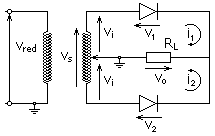
\includegraphics[width=0.6\textwidth]{rectificador}
	\caption{Circuito para hacer un rectificador.}
	\label{fig: rectificador}
\end{figure}

Los dos circuitos equivalentes que se obtienen cuando la fuente de voltaje toma valores positivos y negativos se muestran en las figuras \ref{fig: fuente positiva} y \ref{fig: fuente negativa} respectivamente. \\

\begin{figure}[h!]
	\centering
	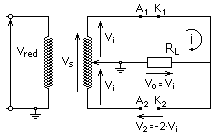
\includegraphics[width=0.6\textwidth]{positiva}
	\caption{Circuito para la fuente de voltaje con valor positivo.}
	\label{fig: fuente positiva}
\end{figure}

\begin{figure}[h!]
	\centering
	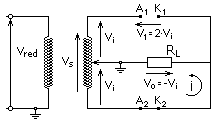
\includegraphics[width=0.6\textwidth]{negativa}
	\caption{Circuito para la fuente de voltaje con valor negativo.}
	\label{fig: fuente negativa}
\end{figure}
	
OJO - FALTA PONER LO DELKIT Y LAS GRÁFICAS, TODO LO SAQUÉ DE WIKIPEDIA ASÍ QUE DEBE ESTAR AHÍ. CLARAMENTE HAY QUE CUADRAR LAS IMÁGENES CUANDO USTED PONGA LO QUE FALTA\\\\\\

\section{Transistores}

Un transistor es un tipo de elemento electrónico semiconductor utilizado para amplificar y "voltear" (dar una respuesta a) señales electrónicas. Se compone de un material semiconductor con por lo menos tres terminales para su conexión a un circuito externo. Un voltaje (o una corriente) aplicado a uno de los terminales cambia la corriente a través de las terminales restantes. Dado que la potencia de salida puede ser mayor que la potencia de entrada, un transistor puede amplificar una señal.

A continuación se describen los principales tipos de conductores.

\begin{itemize}
	\item \textbf{Transistores de juntura bipolar (BJT):} Este tipo de transistores se construye sobre monocristales de materiales seminconductores como el germanio, el silicio o el arseniuro de galio. El cristal se dopa de forma muy controlada en tres zonas precisas, n-p-n o p-n-p, dando lugar a dos junturas p-n. La latra del medio siempre corresponde a la base y las otras dos al emisor y al colector, qeu si bien son del mismo tipo y de signo contrario a la base, tienen diferente contaminación entre ellas dado que típicamente el emisor está mucho más dopado que el colector.\\
	
	En un transistor n-p-n, la juntura emisor-base actúa de tal forma que los electrones son inyectados en la zona de la base. Dado que la base es angosta, la mayoría de los electrones se dispersan de la juntura y son trasladados al colector, mientras que una pequeña parte de los mismos se recombina en la base para dar origen a la corriente de base. Controlando el número de electrones que abandonan la base, el número de electrones que entra al colector puede ser controlada. \\
	
	En la figura \ref{fig: transistor1} se puede apreciar uno de estos transistores.
	
	\begin{figure}[h!]
		\centering
		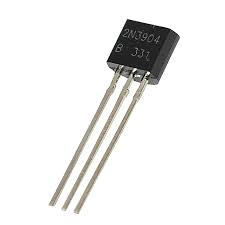
\includegraphics[width=0.25\textwidth]{transistor1}
		\caption{Ejemplo de un transistor BJT.}
		\label{fig: transistor1}
	\end{figure}
	
	\item \textbf{Transistores de efecto campo:} Estos transistores usan electrones o huecos para la conducción. Se caracterizan por tener cuatro terminales denominados denominados source, gate, drain y body, donde típicamente, el body está conectado al source.\\
	
	En estos transistores, la corriente fluye a través de un canal que conecta al drain con la source. La conductividad se varía mediante un campo eléctrico producido cuando se aplica una diferencia de potencial entre las terminales gate y source, por tanto, la corriente qeu fluye entre la drain y la source es controlada por la diferencia de potencial entre las terminales mencionadas previamente.\\
	
	En la figura \ref{fig: transistor2} se puede apreciar uno de estos transistores.
	
	\begin{figure}[h!]
		\centering
		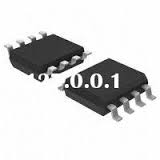
\includegraphics[width=0.25\textwidth]{transistor2}
		\caption{Ejemplo de un transistor de efecto campo.}
		\label{fig: transistor2}
	\end{figure}
	 
\end{itemize}

\end{document}








